% =====================================================================
%  Chapter 4 — Small-Scale Structure
% =====================================================================

\chapter{Small-Scale Structure}
\label{ch:smallscale}

Everything so far has concerned the large scale, where the standard picture
works. The pressure is on the small scale: the distribution of matter inside
individual haloes, the population of satellite galaxies, and the density
profiles of dwarf galaxies. This is where the interesting disagreements are,
and it is where the next decisive constraints are likely to come from.

\section{Three classic problems}The small-scale problems of cold dark matter are
well known and have not gone away.

The \emph{cusp-core problem} is a mismatch of shapes. The standard halo
profile, the Navarro--Frenk--White profile, has a central density that rises
without limit towards the centre, a cusp. Observed rotation curves of dwarf
galaxies, and the stellar density profiles of the Milky Way and Andromeda,
generally prefer a core: a roughly constant central density, or even a
depression. Feedback-driven core formation --- supernova bursts clearing
gas out of the innermost regions and leaving a shallower potential behind ---
is the standard baryonic explanation, and it has support in simulations. It
is also expensive to produce and hard to verify.

The \emph{missing satellites problem} is a mismatch of numbers. Halo models
predict hundreds of subhaloes down to the resolution limit of the simulations;
the observed satellite populations of the Milky Way and Andromeda are far
smaller. The resolution is partial and convincing: many of the predicted
subhaloes are dark and invisible, and the luminous fraction needed is well
below what early simulations produced.

The \emph{too-big-to-fail problem} is the one that survived the others. It
is not about how many satellites there are, but about how dense they are. The
most massive subhaloes in a Milky Way-mass halo are predicted to be far
denser than the observed classical dwarfs. The stated conclusion is that
these subhaloes could not have hosted stars, which would mean the predicted
satellite population is wrong in a way that the number-count argument alone
does not capture.

\section{The soliton}An alternative answer to the core problem is not baryonic at all. In a
field dark matter model with a very small mass, a soliton forms at the
centre of every halo: a stationary, self-bound configuration whose density
rises to a maximum at the origin and then drops as $1/r^4$. Its size is set
by the de Broglie wavelength of the field, and it replaces the cusp.

The Milky Way is the target. De Martino and collaborators argued in 2020
that the soliton should have a mass of order $10^9\ \Msun$, and that the
presence of such a soliton in the Galactic centre is testable by comparing
the gravitational potential inferred from the rotation curve with the
potential inferred from the stellar density distribution \idx{De Martino}. If
the dark matter is a fluid that supports a soliton, the two potentials agree.
If the dark matter is collisionless particles, they do not, because particle
haloes have cusps.

\begin{figure}[!htbp]
\centering
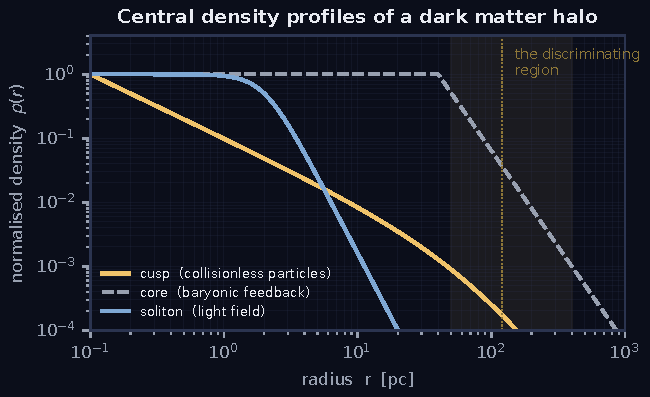
\includegraphics[width=\textwidth]{../figures/fig_smallscale.pdf}
\caption{The central density profile of a dark matter halo under three
assumptions: a cuspy profile as collisionless particles predict, a cored
profile as baryonic feedback can carve, and a soliton profile as a light
field supports. The observationally preferred region is narrow, and the
three curves diverge precisely in the central few hundred parsecs where
the discriminating power lies.}
\label{fig:smallscale}
\end{figure}

\figref{fig:smallscale} shows the three curves and the region in which the
data can distinguish them. The separation is small in the outskirts and
large only in the innermost few hundred parsecs, which is why the test is
hard: it requires the rotation curve of the Milky Way to be known very
precisely in exactly the region where the dust and the gas make it hard.

\section{The counter-evidence}The soliton hypothesis is a live hypothesis and not a
consensus, and the objections are specific and serious.

A 2023 analysis of 153 spiral galaxies found that cored dark matter profiles
are preferred over the soliton-plus-halo configuration in the galaxy
population as a whole, and that the soliton does not improve the fit even in
the systems where it should help most \idx{Wave dark matter rotation curves}.
A separate analysis raised a related problem: the soliton would have to be
excluded from the central regions of dwarf galaxies to fit their observed
density profiles, which requires a mechanism that is not obviously
available, and the resulting soliton--host relation conflicts with the
observed globular cluster systems \idx{Soliton-host relations}.

The cosmological constraint runs the other way. CMB lensing at high
multiplicity measures the mass power spectrum on small scales, and an
ultralight axion with a soliton-forming mass produces a characteristic
suppression that has been searched for and, in 2026, more tightly constrained
\idx{Ultralight axion CMB lensing}. A field that is heavy enough to make a
large soliton --- one that resolves the core problem --- tends to erase the
small-scale power that the lensing data still see.

This is the central tension of the chapter and it is a real one: the same
property that makes a field dark matter attractive, its wavelength, is what
the CMB lensing data limit.

\section{Why this is the discriminating laboratory}The small scale is where the candidate classes make
different predictions. A thermal relic produces cusps and dense satellites. A
light field produces solitons and suppresses satellites. A warm relic with a
specific free-streaming scale produces an intermediate structure. Primordial
black holes produce essentially no low-mass substructure at all, since their
mass function cuts off sharply.

What makes the small scale attractive for the decade ahead is the absence of
an irreducible floor. The neutrino fog that limits direct detection
(Chapter~\ref{ch:direct}) has no analogue here: the limiting factor in
astronomical measurements is systematic --- the difficulty of measuring
stellar velocity fields and distinguishing stars from dark matter in the same
pixel --- and systematic errors can be improved with better instruments and
better data.

\begin{keytakeaways}
\item Cold dark matter has three small-scale problems: the cusp-core
mismatch, the missing satellites, and too-big-to-fail, which is the one that
has not been dissolved.
\item A light boson producing a soliton offers a baryonic-free solution to
the core problem, and the Milky Way's central density profile is the cleanest
test --- with an observationally difficult caveat.
\item The counter-evidence is real: galaxy-scale rotation curves disfavour the
soliton picture, and CMB lensing constrains the ultralight masses that would
produce the largest solitons.
\item Small-scale structure has no neutrino-fog floor, which makes it the most
promising place for the next decisive constraint.
\end{keytakeaways}
